\documentclass[tikz,svgnames]{standalone}

\usepackage{mathtools}

\renewcommand\vec[1]{\boldsymbol{#1}}

\begin{document}
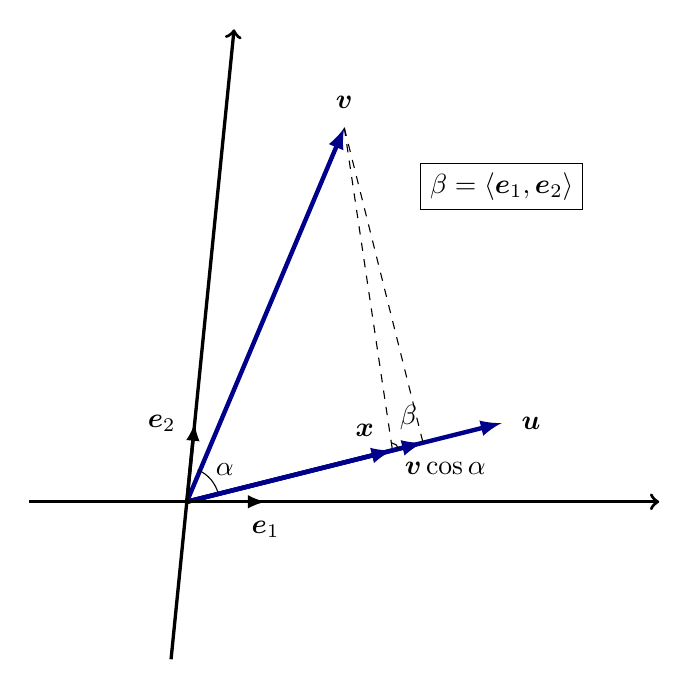
\begin{tikzpicture}[
    vector/.style={ultra thick,-latex,DarkBlue},
    basis/.style={very thick,-latex,Black}
  ]

  \def\xmin{-2} \def\xmax{6}
  \def\ymin{-2} \def\ymax{6}
  \def\gridscale{3}

  \begin{scope}
    \coordinate (origin) at (0,0);
    
    \coordinate (uend) at (4,1);
    \coordinate (vend) at (2,4.75);
    \coordinate (vproju) at (3,0.75);
    \coordinate (vproju2) at (2.611943,0.652986);
    
    \draw [vector] (origin) -- (uend) node [black,right=3] {$\vec u$};
    \draw [vector] (origin) -- (vend) node [black,above=3] {$\vec v$};
    \draw (0.4,0.1) arc[radius = 0.45, start angle= 14.036243, end angle= 67.166346] node [right=3] {$\alpha$};
    
    \draw [dashed] (vend) -- (vproju2);
    \draw [vector] (origin) -- (vproju2) node [black,left=10,above=1] {$\vec x$};
    \draw [dashed] (vend) -- (vproju);
    \draw [vector] (origin) -- (vproju) node [black,right=8,below=3] {$\vec v\cos \alpha$};
    
    \draw (2.689554,0.672388) arc[radius = 0.1, start angle= 14.036243, end angle= 84.289406] node [right=6,above=1] {$\beta$};
    
    \draw (4,4) node[rectangle,draw] {$\beta=\langle\vec e_1,\vec e_2\rangle$};
    
    \pgftransformcm{1}{0}{0.1}{1}{\pgfpoint{0}{0}}
    
    \draw [very thick,->] (\xmin,0) -- (\xmax,0);
    \draw [very thick,->] (0,\ymin) -- (0,\ymax);
    \draw [basis] (origin) -- (1,0) node [below=3] {$\vec e_1$};
    \draw [basis] (origin) -- (0,1) node [left=3] {$\vec e_2$};
  \end{scope}

\end{tikzpicture}
\end{document}